\begin{figure}[t]
\begin{center}
	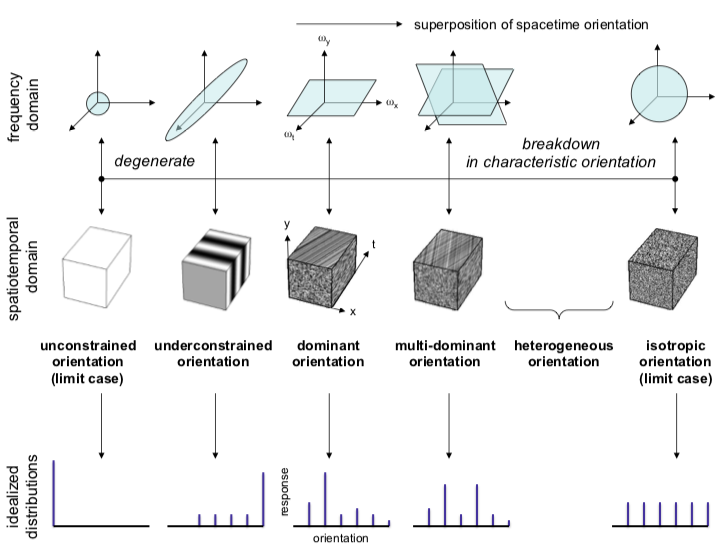
\epsfig{file=spacetime_structures.png, width = \textwidth}\\
	\caption[Spacetime texture spectrum]{Dynamic texture spectrum (adapted from Derpanis \cite{derpanis2012spacetime}). The top and middle rows depict prototypical dynamic textures in the frequency and spatiotemporal domains, respectively. From left-to-right, an increasing amount of spacetime structures are superimposed in a texture. The bottom row depicts a seven bin histogram of the relative spacetime-oriented structure (or lack thereof) present in each dynamic texture. The first histogram bin captures lack of structure. The remaining histogram bins from left-to-right correspond to spacetime orientations selective for static, rightward motion, upward motion, leftward motion, downward motion and flicker structure.}
	\vspace{-0.65cm}
	\label{fig:spacetime_structures}
\end{center}
\end{figure}